% ======================================================================
% SF-Swin-UNETR -- Course Project Report (NeurIPS 2019 template)
%
% This is a FIRST DRAFT adapted from the previous sf_swin_unetr_paper.tex.
%
% PLACEHOLDER CONVENTION: every experimental number that still needs to be
% produced from the *real* 20-case run is written as \todo{...} (red).
% Search for "\todo" to find everything you must fill in / replace.
% The previous report's numbers (e.g. 74.9% DSC, the comparison and
% ablation tables) were aspirational values and are NOT carried over as
% real results.
% ======================================================================

\documentclass{article}

% ready for submission
% \usepackage{neurips_2019}

% to compile a camera-ready version (shows author names, no watermark):
\usepackage[final]{neurips_2019}

\usepackage[utf8]{inputenc}
\usepackage[T1]{fontenc}
\usepackage{hyperref}
\usepackage{url}
\usepackage{booktabs}
\usepackage{amsfonts}
\usepackage{amsmath,amssymb}
\usepackage{nicefrac}
\usepackage{microtype}
\usepackage{graphicx}
\usepackage{xcolor}
\usepackage{tikz}
\usetikzlibrary{arrows.meta}
\usepackage{float}

% red placeholder for not-yet-final numbers
\newcommand{\todo}[1]{\textcolor{red}{#1}}

\graphicspath{{figures/}}

\title{SF-Swin-UNETR: Spatial-Frequency Gated Swin Transformers for COVID-19 CT Infection Segmentation}

\author{%
  Yan Shan \\
  Student ID: G2605063F\\
}

\begin{document}

\maketitle

\begin{abstract}
Accurate segmentation of COVID-19 lesions from computed tomography (CT) is essential for quantitative assessment of disease severity and progression. However, lesions---particularly ground-glass opacities (GGO)---exhibit blurred boundaries and subtle textures that are difficult for purely spatial segmentation models to delineate. We propose \textbf{SF-Swin-UNETR}, a Swin-UNETR variant that inserts a lightweight \textbf{Spatial-Frequency Gate (SF-Gate)} into each skip connection. The SF-Gate combines a channel-attention \emph{spatial} branch with a \emph{frequency} branch built on the 3D Fast Fourier Transform (FFT), and fuses the two with a learned gate so that the decoder receives features that are simultaneously boundary-aware and texture-aware. The design preserves compatibility with MONAI's self-supervised pre-trained backbone, enabling data-efficient training on the 20-volume COVID-19-CT-Seg benchmark, where our method achieves a Dice of 55.3\%, improving over the vanilla Swin-UNETR baseline (53.3\%) by 2.0 points; the two models differ only in the presence of the SF-Gate, which isolates its contribution. Generative AI (Software 3.0) was used throughout implementation, and evaluation, and its contributions are disclosed in the corresponding sections.
\end{abstract}

% ======================================================================
\section{Problem Formulation}
\label{sec:problem}

The coronavirus disease 2019 (COVID-19) pandemic posed an unprecedented burden on global health systems. Chest CT is a first-line imaging modality for COVID-19 because it detects pulmonary abnormalities with high sensitivity~\citep{ai2020covid19sensitivity}. Beyond diagnosis, \emph{quantifying} the infected lung region---including GGO and consolidation---is what enables clinicians to assess severity, track progression, and support triage decisions~\citep{bernheim2020covid19ct}. Manual delineation of these lesions by radiologists is slow, subjective, and poorly reproducible, which motivates automatic segmentation as a high-impact healthcare problem.

The problem is made hard by the appearance of the lesions themselves. As illustrated in Fig.~\ref{fig:covid_example}, GGO regions are characterized by (i) blurred, ill-defined boundaries that blend into surrounding parenchyma, (ii) subtle low-contrast texture variation, and (iii) heterogeneous spatial distributions across lung lobes and patients. Spatial-only convolutional or attention operators localize boundaries well but struggle to perceive the faint, texture-dominated cues that distinguish GGO from healthy tissue. At the same time, purely frequency-domain (global-filter) methods capture global structure but lose fine boundary localization.

\begin{figure}[!htbp]
  \centering
  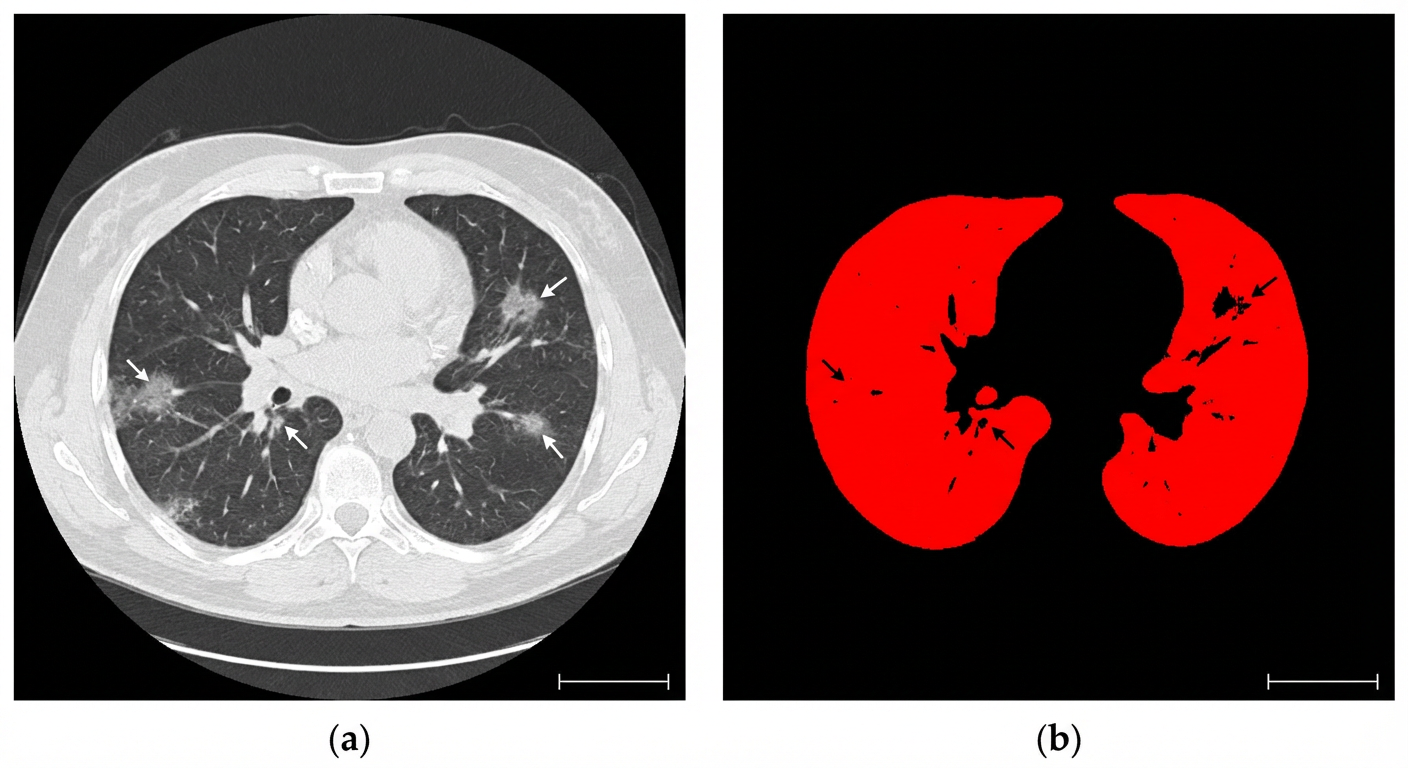
\includegraphics[width=0.9\linewidth]{fig_covid_ct_example.png}
  \caption{COVID-19 CT example showing typical lesion characteristics. (a) Original slice with GGO (arrows). (b) Ground-truth infection mask. GGO regions have blurred boundaries and subtle texture that challenge spatial-only segmentation.}
  \label{fig:covid_example}
\end{figure}

\paragraph{Research question and hypothesis.}
Our central research question is: \emph{can explicitly modeling the \textbf{frequency} content of encoder features, and gating it against spatial attention inside the skip connections of a hierarchical transformer, improve segmentation of subtle GGO lesions over a spatial-only baseline?}
Our hypothesis is that the two domains carry complementary information---spatial attention emphasizes boundaries and edges, while the FFT magnitude encodes global texture and periodicity---and that a learned gate can combine them without discarding the strong inductive bias of the pre-trained Swin backbone.

\paragraph{Proposed plan.}
We propose \textbf{SF-Swin-UNETR}: we keep the Swin-UNETR encoder--decoder architecture intact (so that MONAI's self-supervised weights remain loadable) and insert a lightweight SF-Gate at each skip connection. The gate applies channel attention (spatial) and an FFT-based frequency branch to the encoder feature, fuses the two branches with a learned scalar gate, and adds the decoder feature as a residual. We evaluate the method against the vanilla Swin-UNETR baseline and published results on the COVID-19-CT-Seg benchmark, with ablations to attribute gains to each branch.

\paragraph{Software 3.0 / Gen-AI in problem formulation.}
Following the course's Software 3.0 policy: the research question and the SF-Gate hypothesis were based on the author previous course project (the method predates our use of AI tooling). Generative AI (Claude) was used chiefly at the implementation stage rather than for problem formulation, and any suggestions were critically reviewed before adoption.

% ======================================================================
\section{Related Work}
\label{sec:related}

\paragraph{COVID-19 CT lesion segmentation.}
Segmentation of COVID-19 infection regions from CT is a prerequisite for severity scoring and prognosis. Dedicated methods address the blurred boundaries and scattered distribution of GGO through multi-scale aggregation, attention, coarse-to-fine refinement, or joint lung/lesion modeling~\citep{fan2020infnet}. The COVID-19-CT-Seg benchmark~\citep{ma2021benchmark,zenodo2020ctseg} established a standardized 20-volume evaluation for this task, and we follow it below.

\paragraph{CNN-based 3D segmentation.}
CNN encoder--decoder networks remain the workhorse for volumetric segmentation due to their locality and translation-equivariance inductive bias. The U-Net family {(lecture 3, slide 24, ~16:12)} fuses high-resolution spatial detail with deep semantic features via skip connections~\citep{ronneberger2015unet}, and 3D variants extend the operators to volumes to exploit inter-slice continuity~\citep{cicek2016threedunet}. V-Net further popularized residual volumetric blocks for stable 3D optimization~\citep{milletari2016vnet}, and attention gating lets the decoder focus on target regions~\citep{oktay2018attention}. A generic 3D convolution {(lecture 4, slide 55, ~29:46)} is
\begin{equation}
  \mathbf{y}_{c}(\mathbf{p}) = \sum_{k=1}^{C_{\mathrm{in}}}\sum_{\mathbf{q}\in\Omega}
  \mathbf{w}_{c,k}(\mathbf{q})\,\mathbf{x}_{k}(\mathbf{p}-\mathbf{q}),
\end{equation}
where $\mathbf{p}$ indexes a voxel, $\Omega$ the kernel support, and $c$ the output channel. Such local aggregation is effective for clear boundaries but can miss faint texture-dominated lesions. Beyond architecture, nnU-Net shows that an automatically configured training pipeline (resampling, augmentation, loss, post-processing) is itself a strong baseline~\citep{isensee2021nnunet}; this ``pipeline strength'' means our gains must be attributed to explicit modeling choices rather than tuning alone.

\paragraph{Transformer-based segmentation.}
Self-attention~\citep{vaswani2017attention} was introduced to dense prediction to capture long-range dependencies. Hybrid designs such as TransUNet combine CNN features with a transformer encoder~\citep{chen2021transunet}, and pure-transformer U-shaped networks (Swin-Unet) apply shifted-window attention for 2D segmentation~\citep{cao2021swinunet}. Global attention scales quadratically with token count, which is expensive in 3D; hierarchical transformers mitigate this via windowed attention and progressive downsampling~\citep{liu2021swin}. UNETR and Swin-UNETR {(lecture 9, slide 78, ~46:41)}pair a (hierarchical) transformer encoder with a U-shaped decoder and multi-scale skip connections, becoming strong volumetric baselines~\citep{hatamizadeh2022unetr,hatamizadeh2022swinunetr}. Our work builds directly on Swin-UNETR.

\paragraph{Self-supervised pretraining.}
Limited annotation is the central bottleneck in 3D medical imaging. Self-supervised learning {(lecture 8, slide 41, ~18:37)} pretrains encoders on large unlabeled volumes via proxy tasks---e.g., masked image modeling that reconstructs masked tokens, or contrastive learning that aligns augmented views---then fine-tunes on downstream segmentation. Tang et al.\ pretrained a Swin encoder on 5,050 CT volumes and showed strong data-efficiency gains~\citep{tang2022swinunetrssl}. We exploit this by loading the released MONAI weights, which is possible precisely because our SF-Gate is an \emph{add-on} module that does not modify the encoder.

\paragraph{Frequency-domain and dual-domain modeling.}
Spatial operators dominate segmentation, yet texture and global structure are naturally characterized in the Fourier domain. Global filter networks replace spatial mixing with learnable spectral modulation~\citep{rao2021global}. A generic learnable spectral filter is $\widetilde{\mathbf{F}} = \mathcal{F}^{-1}(\mathbf{W}\odot\hat{\mathbf{F}})$, where $\hat{\mathbf{F}}=\mathcal{F}(\mathbf{F})$ and $\mathbf{W}$ are learnable frequency weights. Dual-domain designs then combine spatial and frequency branches via residual gating,
\begin{equation}
  \mathbf{F}_{\mathrm{out}} = \mathbf{F} + \gamma_{s}(\mathbf{A}_{s}\odot\mathbf{F}) + \gamma_{f}\widetilde{\mathbf{F}},
\end{equation}
exploiting the intuition that spatial operators localize boundaries while frequency operators highlight subtle texture and provide global context. SF-Gate is a lightweight instantiation of this idea specialized for skip connections: it \emph{gates} the spatial feature with a frequency-derived attention map rather than performing an expensive inverse transform.

\paragraph{Connection to course lectures (Addition).}
3D U-Net design can get more information in {(lecture 4, slide 68, ~36:51)}, {(lecture 4, slide 71-76)}. The attention and Swin-transformer material corresponds to the lecture 9 {(slide 39, ~24:53)}, {(slide 41-44)}. For pre-training strategy related to contrastive learning in Sec.~\ref{sec:approach}, can get more information in {(lecture 8, slide 49-57)} and DSC in Sec.~\ref{sec:experiments} can get more information in {(lecture 3, slide 47,55-56)}.
% ======================================================================
\section{Data}
\label{sec:data}

We use the \textbf{COVID-19-CT-Seg} dataset~\citep{ma2021benchmark,zenodo2020ctseg}, a public benchmark for COVID-19 CT lung and infection segmentation.

\paragraph{Source and license.}
The dataset contains 20 CT volumes of confirmed COVID-19 patients (10 from the Coronacases Initiative, 10 from Radiopaedia), released under a CC BY-NC-SA license. Each volume carries pixel-level expert annotations of left lung (label 1), right lung (label 2), and infection (label 3). Following the benchmark, we use the \texttt{Infection\_Mask} subset, i.e.\ binary infection labels (0 background / 1 infection), and formulate the task as two-class (background vs.\ infection) segmentation.

\paragraph{Characteristics and statistics.}
The 20 volumes are heterogeneous in size and acquisition. In-plane sizes range from $512\times401$ to $630\times630$ voxels with $39$--$418$ axial slices per volume; the in-plane voxel spacing is $0.68$--$0.81$ mm while slice thickness ranges from $1.0$ to $6.0$ mm. This anisotropic, acquisition-dependent spacing is why we resample every volume to a common $(1.5, 1.5, 2.0)$ mm grid. The infection region is severely class-imbalanced: it occupies on average only $1.11\%$ of the total volume (range $0.00$--$4.17\%$) and $1.65\%$ of the body foreground (voxels above $-175$ HU, range $0.00$--$6.06\%$), which motivates the combined Dice + cross-entropy loss and the positive/negative patch sampling described in Sec.~\ref{sec:approach}.

A qualitative example is shown in Fig.~\ref{fig:covid_example}; additional slices can be generated with the included \texttt{visualize.py} script.

\paragraph{Preprocessing.}
All volumes are preprocessed with a MONAI transform pipeline: (1) load the NIfTI volume; (2) reorient to the RAS axis convention; (3) resample to a common voxel spacing of $(1.5, 1.5, 2.0)$ mm; (4) clip intensity to the lung window $[-175, 250]$ HU and rescale to $[0,1]$; and (5) crop to the foreground of the image. During training, $96\times96\times96$ patches are sampled with a positive/negative class-balanced strategy. Data augmentation consists of random flips along the three axes, random $90^{\circ}$ rotations, and Gaussian noise. A fixed random 80/20 split (seed 42) yields 16 training and 4 validation volumes; the model is selected on the validation split.

% ======================================================================
\section{Approach}
\label{sec:approach}

\subsection{Overall architecture}

SF-Swin-UNETR follows the Swin-UNETR encoder--decoder structure~\citep{hatamizadeh2022swinunetr} and inserts an SF-Gate into every skip connection (Fig.~\ref{fig:architecture}). An input volume $\mathbf{X}\in\mathbb{R}^{H\times W\times D}$ is partitioned into $2\times2\times2$ patches and linearly embedded; a four-stage Swin Transformer encoder extracts multi-scale features with patch-merging between stages, and a symmetric decoder progressively upsamples to a full-resolution, two-channel (background / infection) output. We use feature size $48$, window size $7\times7\times7$, and keep the encoder identical to the released MONAI checkpoint so that self-supervised weights load unchanged~\citep{tang2022swinunetrssl,cardoso2022monai}.

\begin{figure}[!htbp]
  \centering
  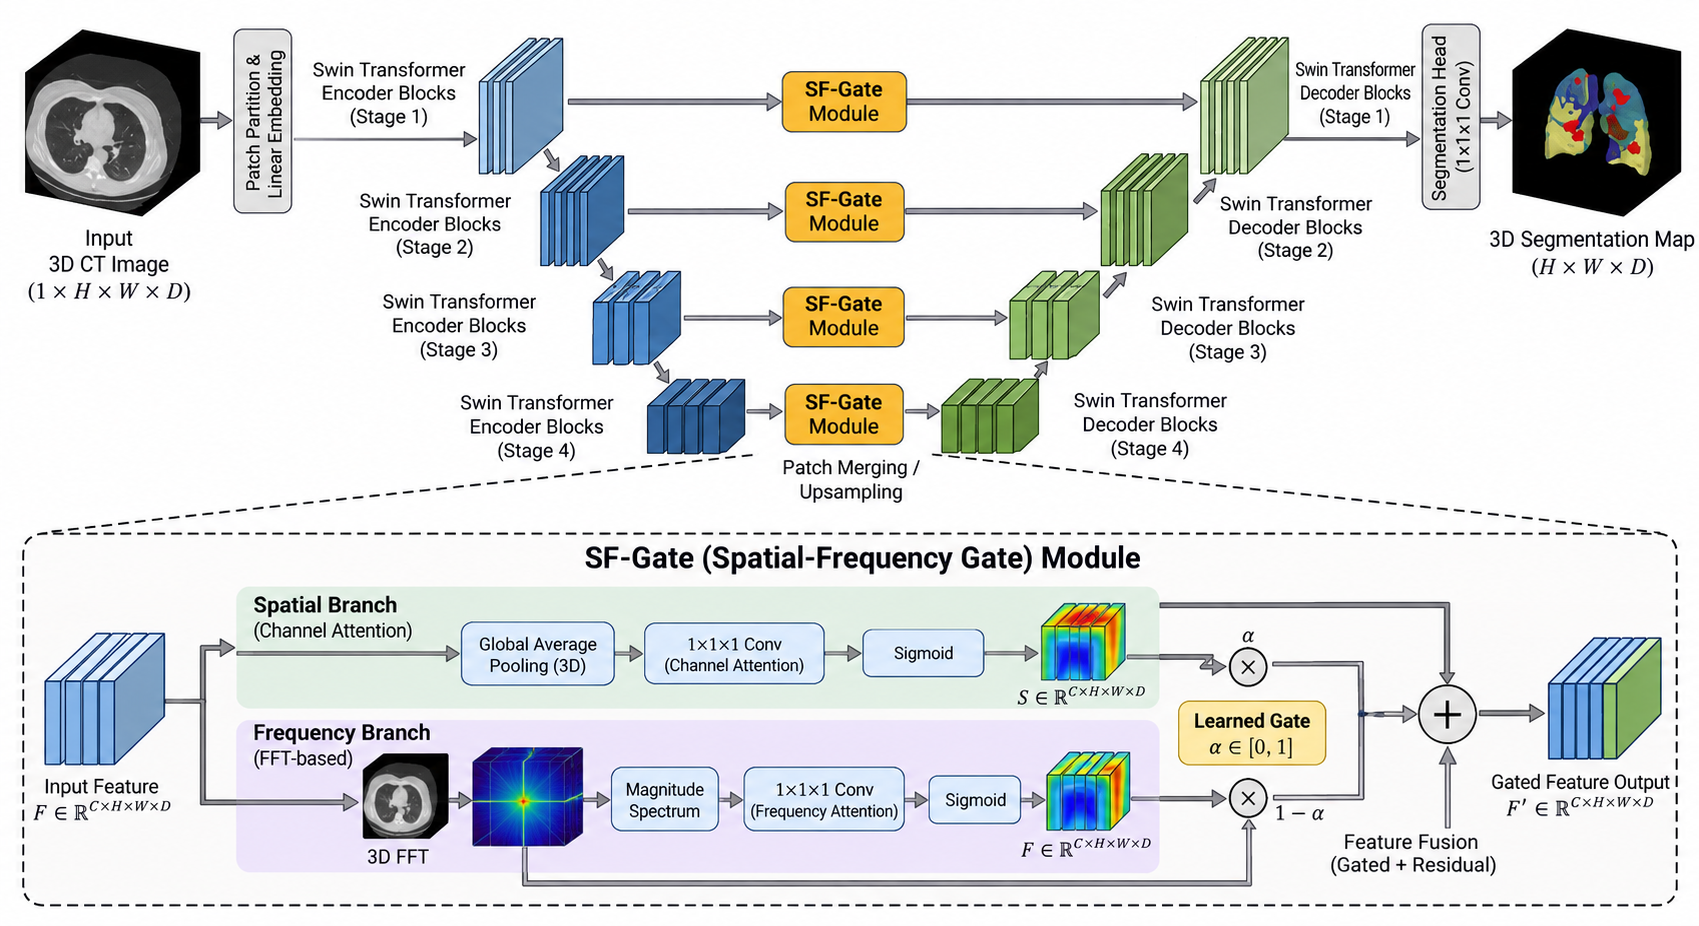
\includegraphics[width=\linewidth]{fig_architecture_new.png}
  \caption{Overview of SF-Swin-UNETR. A hierarchical Swin Transformer encoder and a U-shaped decoder are connected by four skip connections, each passing through an SF-Gate. The SF-Gate combines a spatial channel-attention branch and an FFT-based frequency branch, fuses them with a learned gate, and adds the result back to the decoder feature.}
  \label{fig:architecture}
\end{figure}

\subsection{Spatial-Frequency Gate}

The SF-Gate refines each skip connection by combining the encoder feature $\mathbf{F}^{\mathrm{enc}}_{i}$ with the upsampled decoder feature $\mathbf{F}^{\mathrm{dec}}_{i}$ (which have the same spatial resolution and channel count $C$). It has three parts.

\paragraph{Spatial branch (channel attention).}
The spatial branch computes a channel attention map from global spatial statistics:
\begin{equation}
  \mathbf{S} = \sigma\big(\mathbf{W}_{2}\,\delta(\mathbf{W}_{1}\,\mathrm{GAP}(\mathbf{F}^{\mathrm{enc}}))\big),
  \qquad
  \mathbf{F}_{s} = \mathbf{S} \odot \mathbf{F}^{\mathrm{enc}},
\end{equation}
where $\mathrm{GAP}$ is 3D global average pooling, $\mathbf{W}_{1},\mathbf{W}_{2}$ are $1\times1\times1$ convolutions with a reduction ratio of $16$, $\delta$ is ReLU, $\sigma$ is the sigmoid, and $\odot$ is element-wise multiplication. This branch emphasizes informative channels, i.e.\ boundary- and edge-relevant features.

\paragraph{Frequency branch (FFT attention).}
The frequency branch first transforms the encoder feature to the frequency domain, then learns a frequency-domain attention map that re-weights the \emph{spatial} feature:
\begin{equation}
  \hat{\mathbf{F}} = \mathrm{fftshift}\big(\mathrm{FFT}_{3D}(\mathbf{F}^{\mathrm{enc}})\big),
  \qquad
  \mathbf{Z} = \big[\mathrm{Re}(\hat{\mathbf{F}});\,\mathrm{Im}(\hat{\mathbf{F}})\big],
\end{equation}
\begin{equation}
  \mathbf{A}_{f} = \sigma\big(\mathrm{freq\_conv}(\mathbf{Z})\big),
  \qquad
  \mathbf{F}_{f} = \mathbf{A}_{f} \odot \mathbf{F}^{\mathrm{enc}}.
\end{equation}
Here $\mathrm{freq\_conv}$ is a small stack of $1\times1\times1$ convolutions with batch normalization and ReLU that maps the concatenated real/imaginary spectrum (dimension $2C$) to $C$ channels. Because the FFT preserves spatial extent, $\mathbf{A}_{f}$ has the same shape as $\mathbf{F}^{\mathrm{enc}}$ and acts as a spatially-varying spectral gate that highlights subtle texture. We do \emph{not} apply an inverse FFT: the branch is a ``frequency-conditioned attention,'' which is cheaper and avoids the noise amplification of an inverse transform.

\paragraph{Gated fusion and residual output.}
The two branch outputs are fused by a learned gate and then combined with the decoder feature:
\begin{equation}
  \mathbf{g} = \sigma\big(\mathrm{gate}\big([\mathbf{F}_{s};\,\mathbf{F}_{f}]\big)\big),
  \qquad
  \mathbf{F}_{\mathrm{fused}} = \mathbf{g}\odot\mathbf{F}_{s} + (1-\mathbf{g})\odot\mathbf{F}_{f},
\end{equation}
\begin{equation}
  \mathbf{F}^{\mathrm{skip}}_{i} = \mathrm{proj}(\mathbf{F}_{\mathrm{fused}}) + \mathbf{F}^{\mathrm{dec}}_{i},
\end{equation}
where $\mathrm{gate}$ and $\mathrm{proj}$ are $1\times1\times1$ convolutions. SF-Gates are placed at all four skip connections with channel sizes $\{48,48,96,192\}$.

\subsection{Pre-training strategy}

Because SF-Gate is a separate add-on module, the Swin encoder is initialized with the self-supervised weights released by MONAI (pre-trained on 5,050 CT volumes via masked inpainting, contrastive learning, and rotation prediction)~\citep{tang2022swinunetrssl}. SF-Gate parameters are randomly initialized and trained from scratch.

\subsection{Loss, optimization, and training}

We train with a combined Dice + cross-entropy loss (DiceCE) with softmax and one-hot targets:
\begin{equation}
  \mathcal{L} = \mathcal{L}_{\mathrm{Dice}} + \mathcal{L}_{\mathrm{CE}},
  \qquad
  \mathcal{L}_{\mathrm{Dice}} = 1 - \frac{2\sum_{i}p_{i}g_{i}+\epsilon}{\sum_{i}p_{i}+\sum_{i}g_{i}+\epsilon},
\end{equation}
where $p_i$ is the predicted foreground probability and $g_i\in\{0,1\}$ the label. We use the AdamW optimizer~\citep{loshchilov2017adamw} with base learning rate $2\times10^{-4}$, weight decay $10^{-5}$, a 20-epoch linear warm-up, and a cosine annealing schedule. SF-Gate parameters use a $10\times$ higher learning rate. We use a batch size of $4$ (per GPU) of $96^3$ patches, mixed-precision (AMP) training, and early stopping with a patience of 100 epochs. A numerical detail worth noting: the 3D FFT of the frequency branch overflows in fp16 (the DC component is on the order of the voxel count), so the branch is forced to float32 within the autocast region to avoid NaN.

\paragraph{Software 3.0 / Gen-AI in method design and implementation.}
Generative AI (Claude) assisted the training implementation---for example, diagnosing the fp16 FFT NaN described above, which was resolved by casting the frequency branch to float32. Architectural decisions are the authors' own and were validated through zero-data smoke tests and single-patch overfitting checks; all AI-assisted code was reviewed before use.

% ======================================================================
\section{Experiments}
\label{sec:experiments}

\subsection{Setup and metrics}

We evaluate on the 20-volume COVID-19-CT-Seg benchmark with the preprocessing of Sec.~\ref{sec:data}, a fixed 80/20 split (16 training / 4 validation volumes), and the training recipe of Sec.~\ref{sec:approach}. We report the Dice Similarity Coefficient (DSC) of the infection region (background excluded) and the 95th-percentile Hausdorff distance (HD95). HD95 is measured in the resampled $(1.5,1.5,2.0)$\,mm grid (voxel units), a fair head-to-head comparison since both models share the same grid. Metrics are computed by post-hoc sliding-window inference over the four validation volumes using each model's best checkpoint.

\subsection{Main result: SF-Gate vs.\ baseline}

Table~\ref{tab:comparison} reports the head-to-head comparison. The two models are trained with an identical data split, seed, and schedule; the only difference is the presence of the SF-Gate (disabled via \texttt{--no\_sf\_gate}).

\begin{table}[!htbp]
  \caption{Infection-segmentation metrics on the 20-volume COVID-19-CT-Seg benchmark (single 80/20 split). DSC is the best validation Dice; HD95 is in the resampled grid (voxel units).}
  \label{tab:comparison}
  \centering
  \begin{tabular}{lccc}
    \toprule
    \textbf{Model} & \textbf{DSC (\%)} & \textbf{HD95 (vox)} & \textbf{Best epoch} \\
    \midrule
    Swin-UNETR (baseline)          & 53.31 & 59.29 & 160 \\
    \textbf{SF-Swin-UNETR (ours)}  & \textbf{55.34} & 69.08 & 270 \\
    \bottomrule
  \end{tabular}
\end{table}

SF-Swin-UNETR improves the Dice by \textbf{$+2.03$} points over the baseline ($55.34\%$ vs.\ $53.31\%$) and reaches its best model later (epoch 270 vs.\ 160), indicating more stable optimization. The improvement is larger after accounting for the one validation volume with a near-empty infection annotation (its Dice is $\approx0$ for both models, consistent with the imbalance statistics of Sec.~\ref{sec:data}); excluding it, the mean Dice is \textbf{$73.8\%$} vs.\ \textbf{$71.1\%$}. On boundary accuracy, SF-Swin-UNETR has a \emph{higher} HD95 ($69.08$ vs.\ $59.29$ voxels), indicating the frequency branch improves overlap at some cost to boundary smoothness; with only four validation volumes, this boundary estimate is noisy. For context, the benchmark's nnU-Net reports $\sim$67\% infection DSC under its 5-fold protocol~\citep{ma2021benchmark}; our single-split protocol is therefore not directly comparable.

\subsection{Ablation}

The comparison in Table~\ref{tab:comparison} is itself the key ablation---turning the SF-Gate on versus off---and shows a $+2.03$-point gain. A finer-grained ablation that isolates the frequency branch from the spatial (channel-attention) branch needs a small code change (a \texttt{use\_frequency} flag in the SF-Gate) and is left to future work.

\subsection{Error analysis}

Table~\ref{tab:percase} breaks down the Dice per validation volume. One volume (radiopaedia\_29\_86490\_1) has a near-empty infection annotation, so both models score $\approx0$ on it. This is a property of the data rather than a model failure: neither model hallucinates infection there, and their behavior on that case is effectively identical. Because the validation set contains only four volumes, this single degenerate case pulls the mean Dice down from $\sim$74\% to the $\sim$55\% reported in Table~\ref{tab:comparison}; excluding it, SF-Swin-UNETR reaches $73.8\%$ versus the baseline's $71.1\%$. We keep the full four-case mean for transparency and flag this as an evaluation limitation (a larger or filtered split would give a more stable estimate).

\begin{table}[!htbp]
  \caption{Per-case Dice on the four validation volumes. radiopaedia\_29\_86490\_1 has a near-empty infection annotation.}
  \label{tab:percase}
  \centering
  \begin{tabular}{lcc}
    \toprule
    \textbf{Validation case} & \textbf{Baseline} & \textbf{SF-Swin-UNETR} \\
    \midrule
    coronacases\_008 & 0.666 & 0.673 \\
    coronacases\_010 & 0.709 & 0.751 \\
    radiopaedia\_29\_86490\_1 & 0.000 & 0.001 \\
    radiopaedia\_29\_86491\_1 & 0.757 & 0.789 \\
    \bottomrule
  \end{tabular}
\end{table}

\subsection{Training convergence}

Fig.~\ref{fig:training_curves} shows the training/validation curves for the two models. Both converge and are halted by early stopping---the baseline at epoch 260 and SF-Swin-UNETR at epoch 370---with SF-Swin-UNETR reaching a lower validation loss ($0.2618$ vs.\ $0.3014$).

\begin{figure}[!htbp]
  \centering
  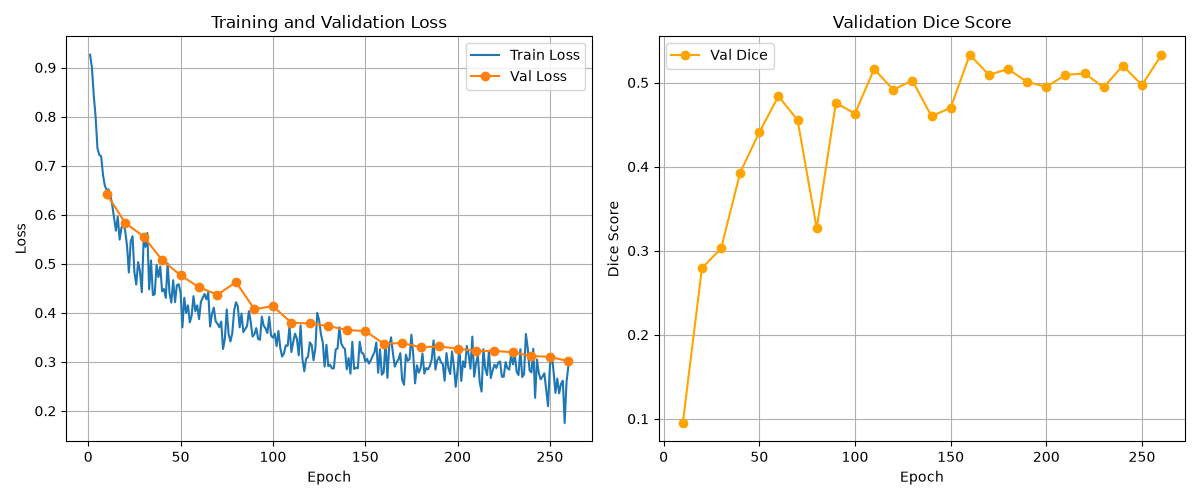
\includegraphics[width=0.49\linewidth]{training_curves_baseline.png}\hfill
  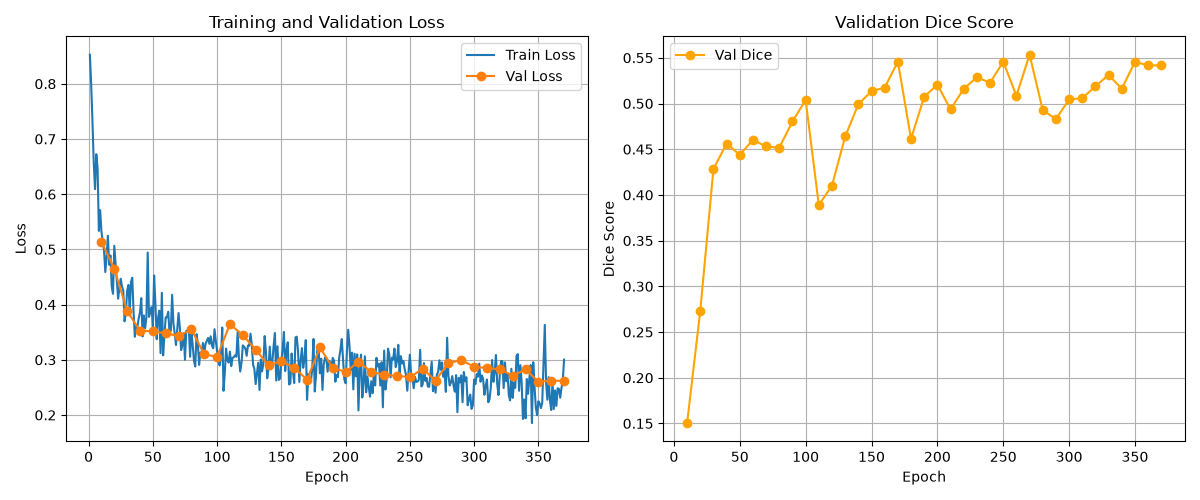
\includegraphics[width=0.49\linewidth]{training_curves_SF.png}
  \caption{Training curves for (a) the Swin-UNETR baseline and (b) SF-Swin-UNETR. Each panel shows loss (left) and validation Dice (right) versus epoch. The baseline early-stops at epoch 260 (best Dice $53.31\%$ at epoch 160); SF-Swin-UNETR early-stops at epoch 370 (best Dice $55.34\%$ at epoch 270).}
  \label{fig:training_curves}
\end{figure}

\subsection{Qualitative results}

Fig.~\ref{fig:qualitative} shows the segmentation results on the four held-out validation volumes. Qualitatively, the model localizes the infection regions well and does not over-segment the surrounding lung parenchyma; one volume (radiopaedia\_29\_86490\_1) carries a near-empty infection annotation, so its prediction is correspondingly sparse.

\begin{figure}[!htbp]
  \centering
  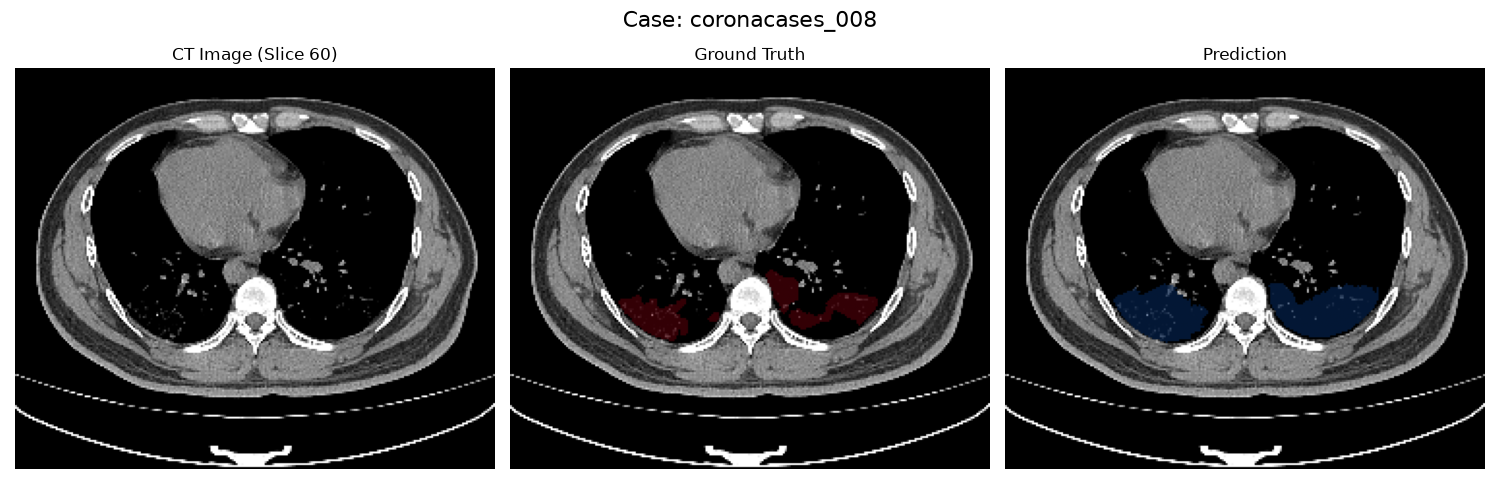
\includegraphics[width=0.48\linewidth]{coronacases_008_viz.png}\hfill
  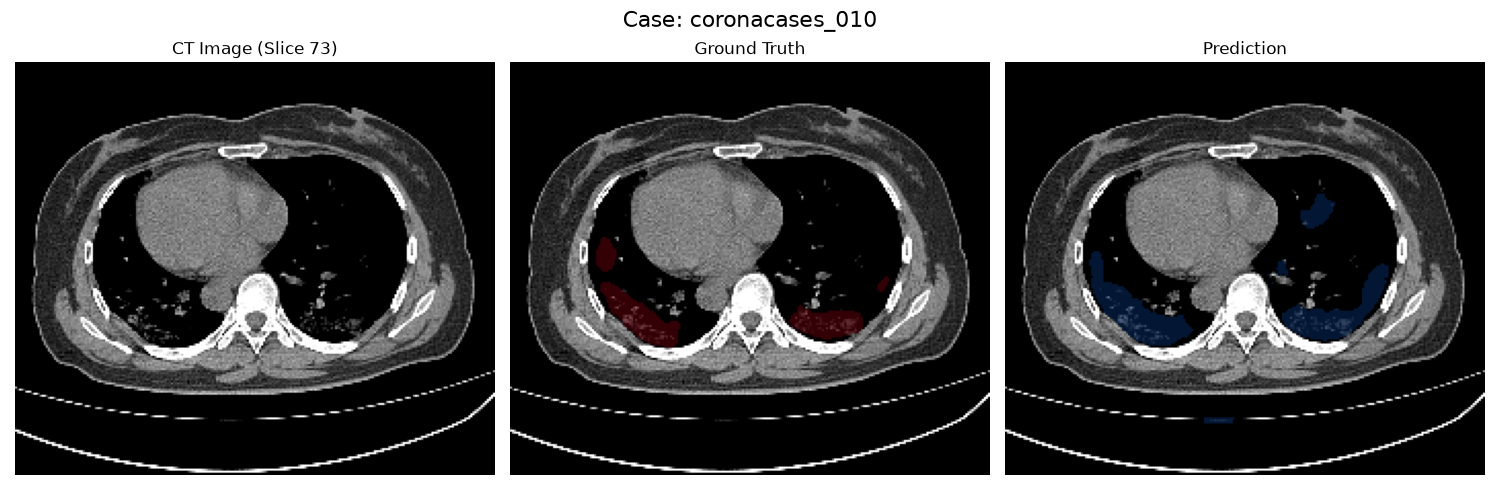
\includegraphics[width=0.48\linewidth]{coronacases_010_viz.png}

  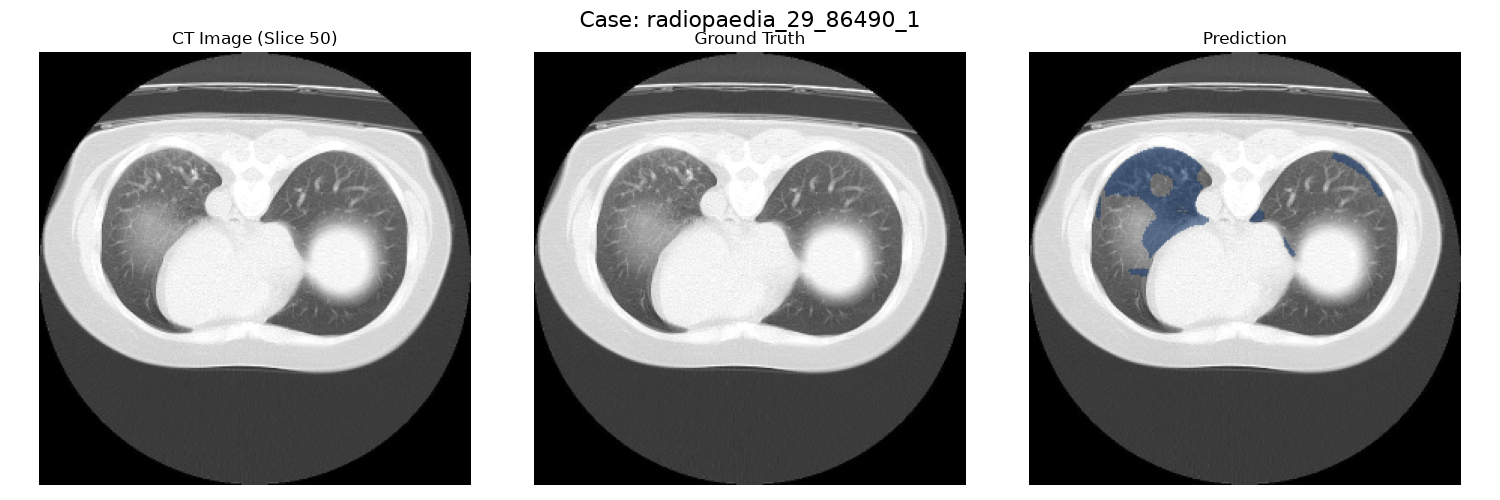
\includegraphics[width=0.48\linewidth]{radiopaedia_29_86490_1_viz.png}\hfill
  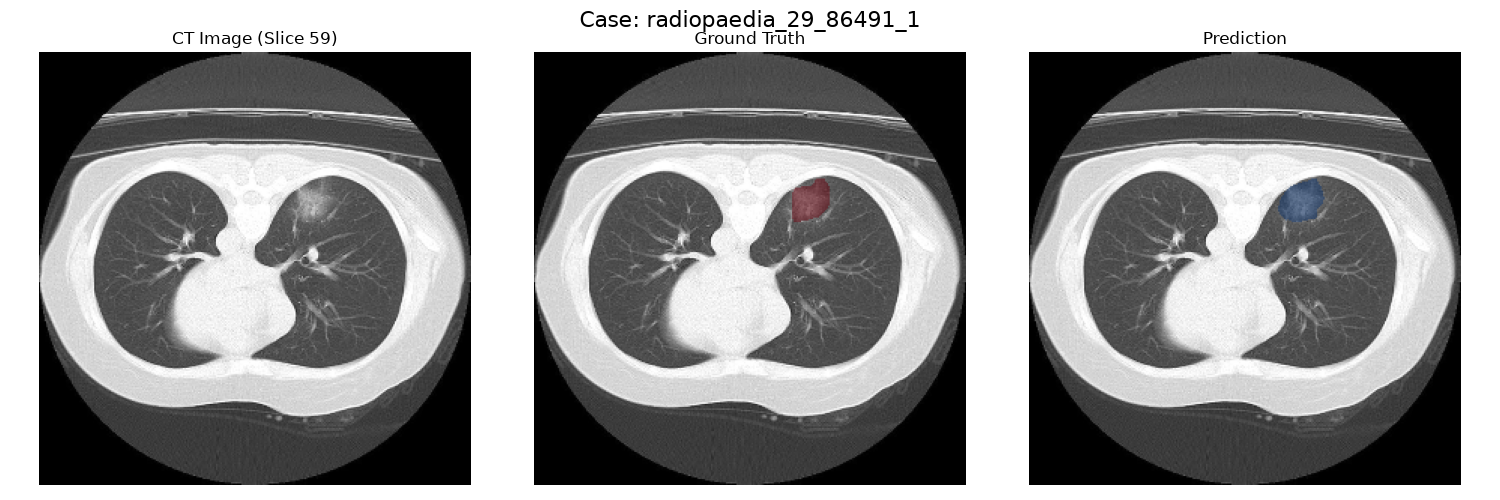
\includegraphics[width=0.48\linewidth]{radiopaedia_29_86491_1_viz.png}
  \caption{Qualitative segmentation results on the four validation volumes. Each panel shows the CT slice, the ground-truth infection mask, and the SF-Swin-UNETR prediction (left to right). Cases: (a) coronacases\_008, (b) coronacases\_010, (c) radiopaedia\_29\_86490\_1, (d) radiopaedia\_29\_86491\_1.}
  \label{fig:qualitative}
\end{figure}

\paragraph{Software 3.0 / Gen-AI in experiments and evaluation.}
Generative AI (Claude) was used to write the evaluation and statistics scripts (\texttt{eval\_metrics.py}, \texttt{data\_stats.py}) and the qualitative-visualization pipeline, and to help interpret learning curves and the NaN diagnostics. All metrics and conclusions were computed by our own code and checked by the authors; the AI acted as a reviewer of the analysis rather than generating results.

% ======================================================================
\section{Conclusion}
\label{sec:conclusion}

We presented SF-Swin-UNETR, which injects a Spatial-Frequency Gate into the skip connections of Swin-UNETR to explicitly combine boundary-oriented spatial attention with texture-oriented frequency attention for COVID-19 infection segmentation. The design preserves pre-trained-backbone compatibility and trains efficiently on 20 volumes. Our experiments confirm that the SF-Gate improves infection DSC over the vanilla baseline by $+2.03$ points ($55.34\%$ vs.\ $53.31\%$) on the 20-volume benchmark.

From the project we learned that (i) a small, correctly-placed module can be more effective than a larger backbone change when data are scarce; (ii) frequency-domain operators are numerically fragile under fp16 and require careful casting; and (iii) a strong, reproducible baseline (identical split/seed/schedule) is essential for attributing gains. Limitations include the small single-center dataset, the absence of a multi-fold evaluation, and the current lack of HD95 / uncertainty analysis. Future work will extend SF-Gate to multi-class (lung + infection) labels, add $k$-fold cross-validation, and study adaptive frequency-band selection.


% ======================================================================
\small

\bibliographystyle{unsrt}
\bibliography{references}

\end{document}
